\chapter{Point Cloud Compression}
\label{ch:compression}
This Chapter present the last subject of the internship, \emph{point cloud compression}. Section~\ref{sc:spec-compression} gives a lead on the context bringing such need. Then, Section~\ref{sc:work-compression} mentions notable previously-published work on the subject. In Section~\ref{sc:custom-compression} we describe a custom approach. The benchmark result highlights the relevance of Zip Compression to our objectives. Therefore, in the final Section~\ref{sc:integration}, we discuss about \emph{Zip compression} integration to \CC.

\section{Specifications}
\label{sc:spec-compression}

\subsection{Context}
As said in the introduction, \CC provides a cloud service for client not having performant machines. When a client submit a job, at some point, data uploading starts including the point cloud (if available\footnote{The reconstruction can also be made with photos.}). If the upload fails due to lost internet connection or any other reason, the upload restarts from scratch. Many point clouds are huge with a file size over $10$ GB, some of them more than $100$ GB. A Point cloud
easily becomes the biggest part of the data being upload to the cloud service. Therefore, reducing its size before uploading it, is a first good step toward better cloud services. This is where the scope of this work ends. A second step would probably be to find a way to send data through streaming with a recovery system on the cloud in case of fail.

This is how the need for \emph{Point Cloud Compression} emerged. In the final solution integration described in Section~\ref{sc:integration}, we compress not only point clouds but also XML files. When exporting a \emph{block}\footnote{An isolated instance of work in a \CC project}, \CC dumps an XML with necessary information for later uploadings. The size of this XML can grow fast based on the project's size and complexity. But this XML compression was not on purpose at the beginning.

\subsection{Objective}
The method of compression must observe the following rules:
\begin{itemize}
  \item take as input any point cloud, provided it is static.
  \item being preferably lossless, points location errors are tolerated under 1mm precision,
  \item being able to compress several fields such as: point locations, normals, colors, intensity,
  \item compress the point cloud size ideally by two (2),
  \item have a reasonable compressing time such that the uploading time saved thanks to file size reduction is not lost during point cloud compression.
\end{itemize}

\section{Related work}
\label{sc:work-compression}
This section introduces different approach for point cloud compression. There is a need for clarification. The term \emph{point cloud compression} generally refers to ingenious representations of point clouds such that they take less space and can be easily loaded and used. However, for easy readability purposes we also use \emph{point cloud compression} to refer to simple arithmetic compression even if they are applied without no context of what is being compressed.

Some point cloud compression algorithms compress the underlying mesh instead of the point cloud itself, such as: \cite{gumhold2, rossignac}. Computing the underlying mesh would take more time. In the \cite{gumhold} approach, they encode the point cloud in a prediction tree. This tree that predicts next points based on previous one is the only thing dumped as a file, thus this method does not treat colors, normals or any other information that can be find in a point cloud. Traditional schemes uses octree data structures. For instance \cite{schnabel, huang} propose to compress the point cloud with an octree decomposition of space. The child cell configurations are coded in a predictive way based on a local surface approximation. More recently, \cite{zhang} propose a way to compress generic\footnote{With any point attributes. For instance: normals, colors.} point clouds by building a graph and treat attributes as signals over the graph. The results of this algorithm outperforms the traditional octree-based algorithms. We did not have a chance to further investigate this method because of time.

One of the earliest method adressing efficient point cloud representation is the Qsplat rendering system of \cite{qsplat}. Each node of the point cloud is quantized to fourty-eight (48) bits. Our approach described in Section~\ref{sc:custom-compression} is inspired by this quantization.

\section{A bit-wise compression of point clouds}
\label{sc:custom-compression}
This section describes a custom point cloud compression. It is not exaclty a compression algorithm as it is just a packed representation of the same point cloud used as input to Brotli~\cite{brotli}, a compression algorithm. This method filters point cloud data by ignoring useless data reguardind the needed precision. Section~\ref{subsc:overview-packed} explains how this packed representation is obtained before calling Brotli while Section~\ref{subsc:compression-benchmark} compares it with Brotli itself, 7Z (LZMA) and Zip.

\subsection{Overview}
\label{subsc:overview-packed}
In the Background Chapter of this report, precisely Section~\ref{sc:back-point-cloud} a point $p_i$ is introduced as a tuple $\left\langle x_i, y_i, z_i, \vec{n}_i \right\rangle$ where $i$ is an unique integer identifying $p_i$, ($x_i$, $y_i$ and $z_i$) are the coordinates of $p_i$ and $\vec{n}_i$ is the normal at $p_i$. But, more information can be stored for each point:
\begin{itemize}
\item the $rgb$ colors of the point,
\item its source ID corresponding to the scanner to which the point is assigned,
\item the intensity of the point.
\end{itemize}

This method stores each point on two hundred three (203) or two hundred seven (207) bits (depending on the last bullet point) instead of five hundred twenty (520) bits :
\begin{itemize}
\item For each point or normal coordinates $x_i$ , $y_i$, $z_i$, $n_i^x$, $n_i^y$ and $n_i^z$ we store its sign on one (1) bit, the integer part on sixteen (16) bits and the decimal part on ten (10) bits. Originally stored as \emph{double} on sixty-four (64) bits, we reduce it to twenty-six (27) bits. Note that this choice has some limitations. Large-scale point clouds need to be divided into pieces before being compressed in order to fit in the integer range.
\item Each of the $rgb$ colors can be stored on height (8) bits as their value is between 0 and 255. They are originally stored as \emph{float} in order to support more color variation. The difference is barely visible to the naked eye.
\item The source ID is stored on five (5) bits, considering there will never be more than thirty-two (32) scanners in a point cloud. It is originally stored as an \emph{uint8\_t}.
\item The intensity is a decimal value in the range $[0, 1]$. It can be stored on two (2) or height (8) bits depending on the presence of the decimal part. If the value is $0$ or $1$, the first bit is set to $1$ and the second bit is the set to the value. But if the value is a number in the range $]0, 1[$, the first bit is set to $0$ and the others represent the decimal part.
\end{itemize}

Once the packed representation of the point cloud is obtained and written on disk, it is given as an input to Brotli~\cite{brotli} algorithm.

\subsection{Comparison with Brotli, 7Z and Zip}
\label{subsc:compression-benchmark}
\begin{sidewaysfigure}
    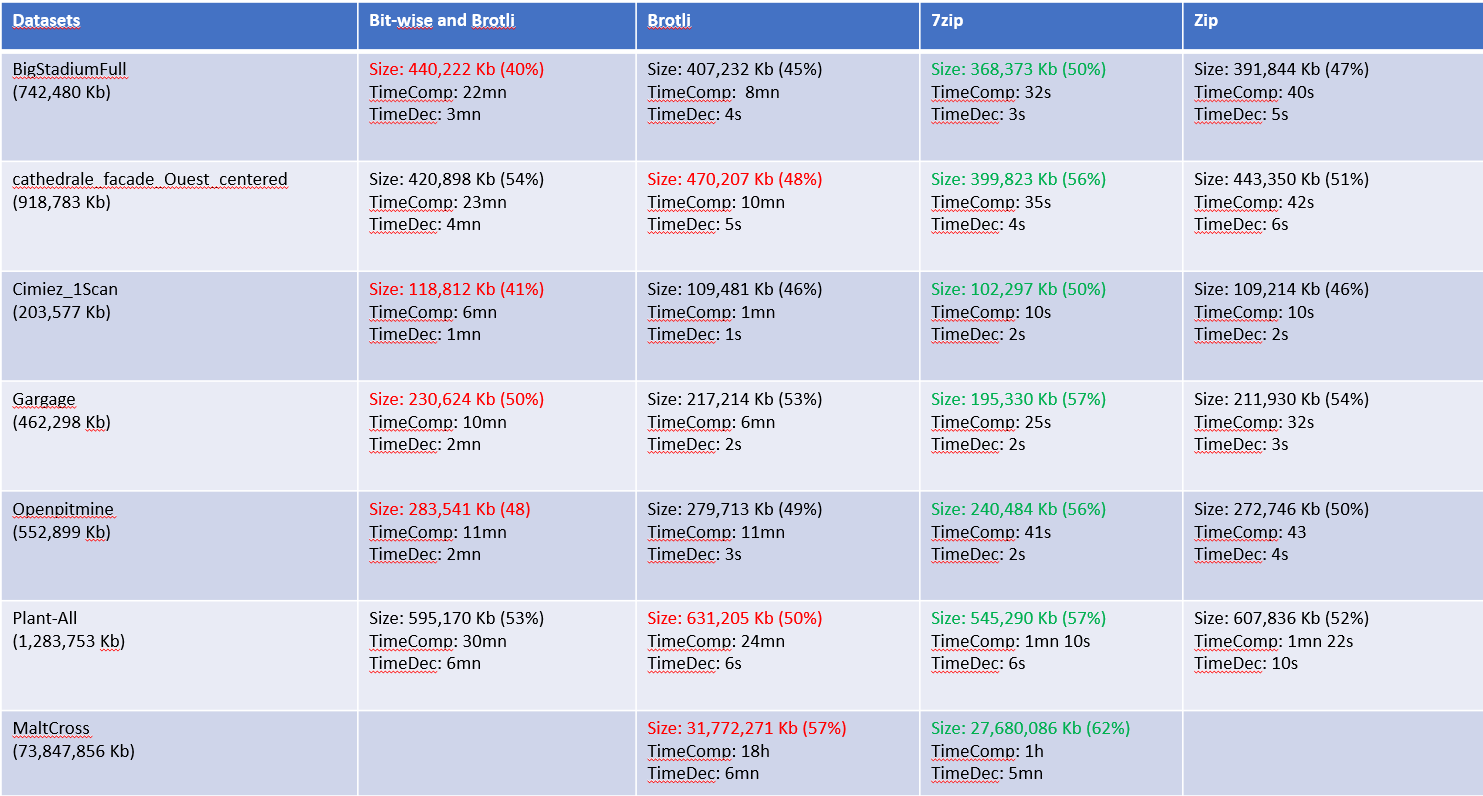
\includegraphics[width=\textwidth]{img/bit-wise-benchmark.png}
    \caption{Benchmark result comparing our method (Bit-wise + Brotli) to Brotli, 7Zip and Zip on different point clouds. For each experience, find the size after compression, the reached compression percentage and both compression and decompression times. This measures are made on a machine with \emph{Intel(R) Xeon(R) CPU E5-1620 v3 @ 3.50 GHz 3.50 GHz} and \emph{64 RAM GB}.}
    \label{fig:bit-wise-benchmark}
\end{sidewaysfigure}

\begin{sidewaysfigure}
    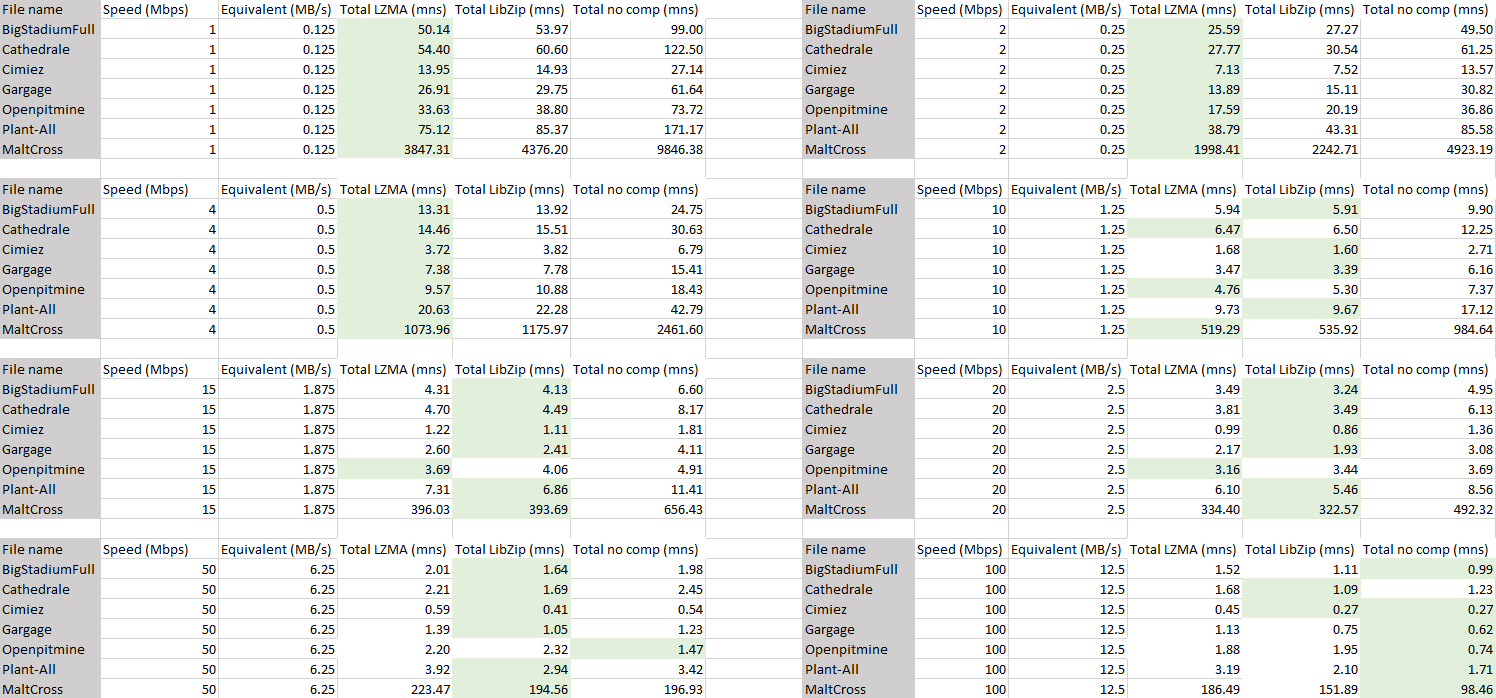
\includegraphics[width=\textwidth]{img/compare1.png}
    \caption{Simulation at different uploading speed and for different point clouds of the total required time to send data to the cloud service: compression time (if any compression) + uploading time. It compares LZMA (7Zip) with Ziplib and the current state of \CC (no compression).}
    \label{fig:compare-excel}
\end{sidewaysfigure}

Figure~\ref{fig:bit-wise-benchmark} shows benchmark result comparing our custom approach (a \emph{bit-wise} compression followed by Brotli) to Brotli itself, 7Zip and Zip. In most point clouds, the combination of the packed representation and Brotli achives slightly better compression results than just Brotli. But the compression times show that any method involving Brotli is not a viable solution for \CC. Brotli takes up to twenty-four (24) minutes to compress a bit more than one (1) GB point cloud file where 7Zip and Zip need around one (1) minute.\\
As 7Zip and Zip licences are compatible with \CC for commercial use, we did futher research on both methods.

Figure~\ref{fig:compare-excel} is a simulation (at different uploading speed value) of the total time to send each of the point clouds on the cluster. Three cases are explored: the current one (no compression), one using LZMA (the 7ZIP algorithm) compression before uploding data and the last one using ZipLib before uploading data. This simulation is based on the real compression times obtained. Find in green the fatest method. At a speed of one (1) Mbps, so a very slow uploading time, LZMA is faster. There is no surprise, at this speed level, compressing data before uploading saves time. But, as the uploading speed grows, reaching usual speed uploading, LibZip starts to be a better solution despite the fact that it does not reach compressing percentage rate of 7ZIP. What surprises us is that here ZipLib is sometimes faster than LZMA (7ZIP) while it was the opposite in the previous experience (Figure~\ref{fig:bit-wise-benchmark}). Using the Zip library instead of the binary seems to be faster. Of course, at very high uploading speed, point cloud compression is a waste of time.

We decided to integrate Zip compression in \CC.

\section{Integration of Zip compression}
\label{sc:integration}
This section describe the integration of Zip compression to \CC. Note that compression is the only one work of this report integrated to \CC. \emph{ScanFinder} and \emph{Disk-based Visibility} are still prototypes.

\paragraph{Code interface}
\begin{figure}
  \centering
  \begin{lstlisting}
  namespace Zip
  {
      bool compress(std::string const& inputPath, std::string const& outputPath,
              zip_progress_callback pf = nullptr, void* pProgressData = nullptr);

      bool decompress(std::string const& inputPath, std::string const& outputPath);
  }
  \end{lstlisting}
  \caption{Function using least-square to fit a line to the given set of points.}
  \label{fig:code-interface}
\end{figure}
ZipLib was already integrated in the third parties of \CC. No new library linkage has been set up. \CC uses ZipLib in a completely different context. We implemented two code interface methods, for easy use of ZipLib. Figure~\ref{fig:code-interface} shows the prototype of both methods. The  \emph{compress} methods can be called with a callback function for monitoring the file compression. This is used for the progression bar appearing when exporting  \emph{blocks} in \CC (see Figure~\ref{fig:export3}).


\paragraph{\CC Software}
\begin{figure}
  \centering
  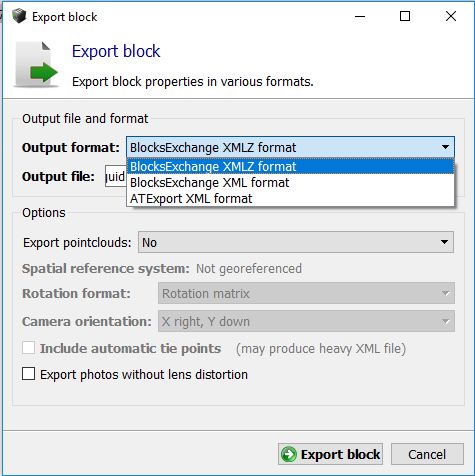
\includegraphics[scale=0.7]{img/export1.png}
  \caption{The new block export dialog of \CC: XMLZ (Zip of XML) format added.}
  \label{fig:export1}
\end{figure}
\begin{figure}
  \centering
  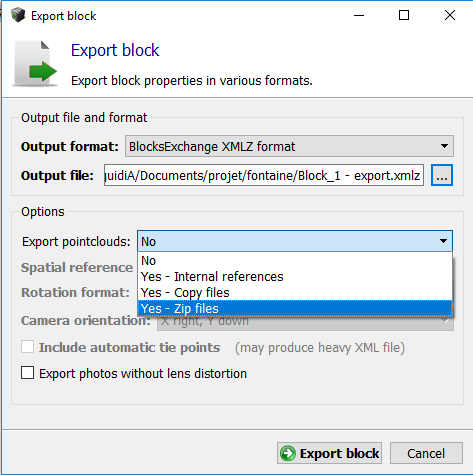
\includegraphics[scale=0.7]{img/export2.png}
  \caption{The new block export dialog of \CC: possibility to Zip files.}
  \label{fig:export2}
\end{figure}
\begin{figure}
  \centering
  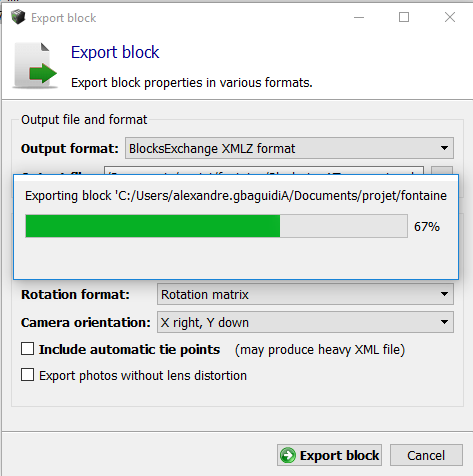
\includegraphics[scale=0.7]{img/export3.png}
  \caption{The new block export dialog of \CC: progress bar.}
  \label{fig:export3}
\end{figure}

Figure~\ref{fig:export1} and Figure~\ref{fig:export2} show visuals of the new feature integrated. Two new possibilities are now available:
\begin{itemize}
\item compress the XML file by selecting \emph{BlocksExchange XMLZ format} (Figure~\ref{fig:export1}),
\item compress the point cloud by selecting \emph{Yes - Zip files} (Figure~\ref{fig:export2}).
\end{itemize}
